%########################################################################################
% Chapter: Wissen in synchronen und asynchronen Systemen
%########################################################################################
\section{Wissen in synchronen und asynchronen Systemen}
\label{sync_vs_async}
%\begin{figure}[H]
%\centering
%      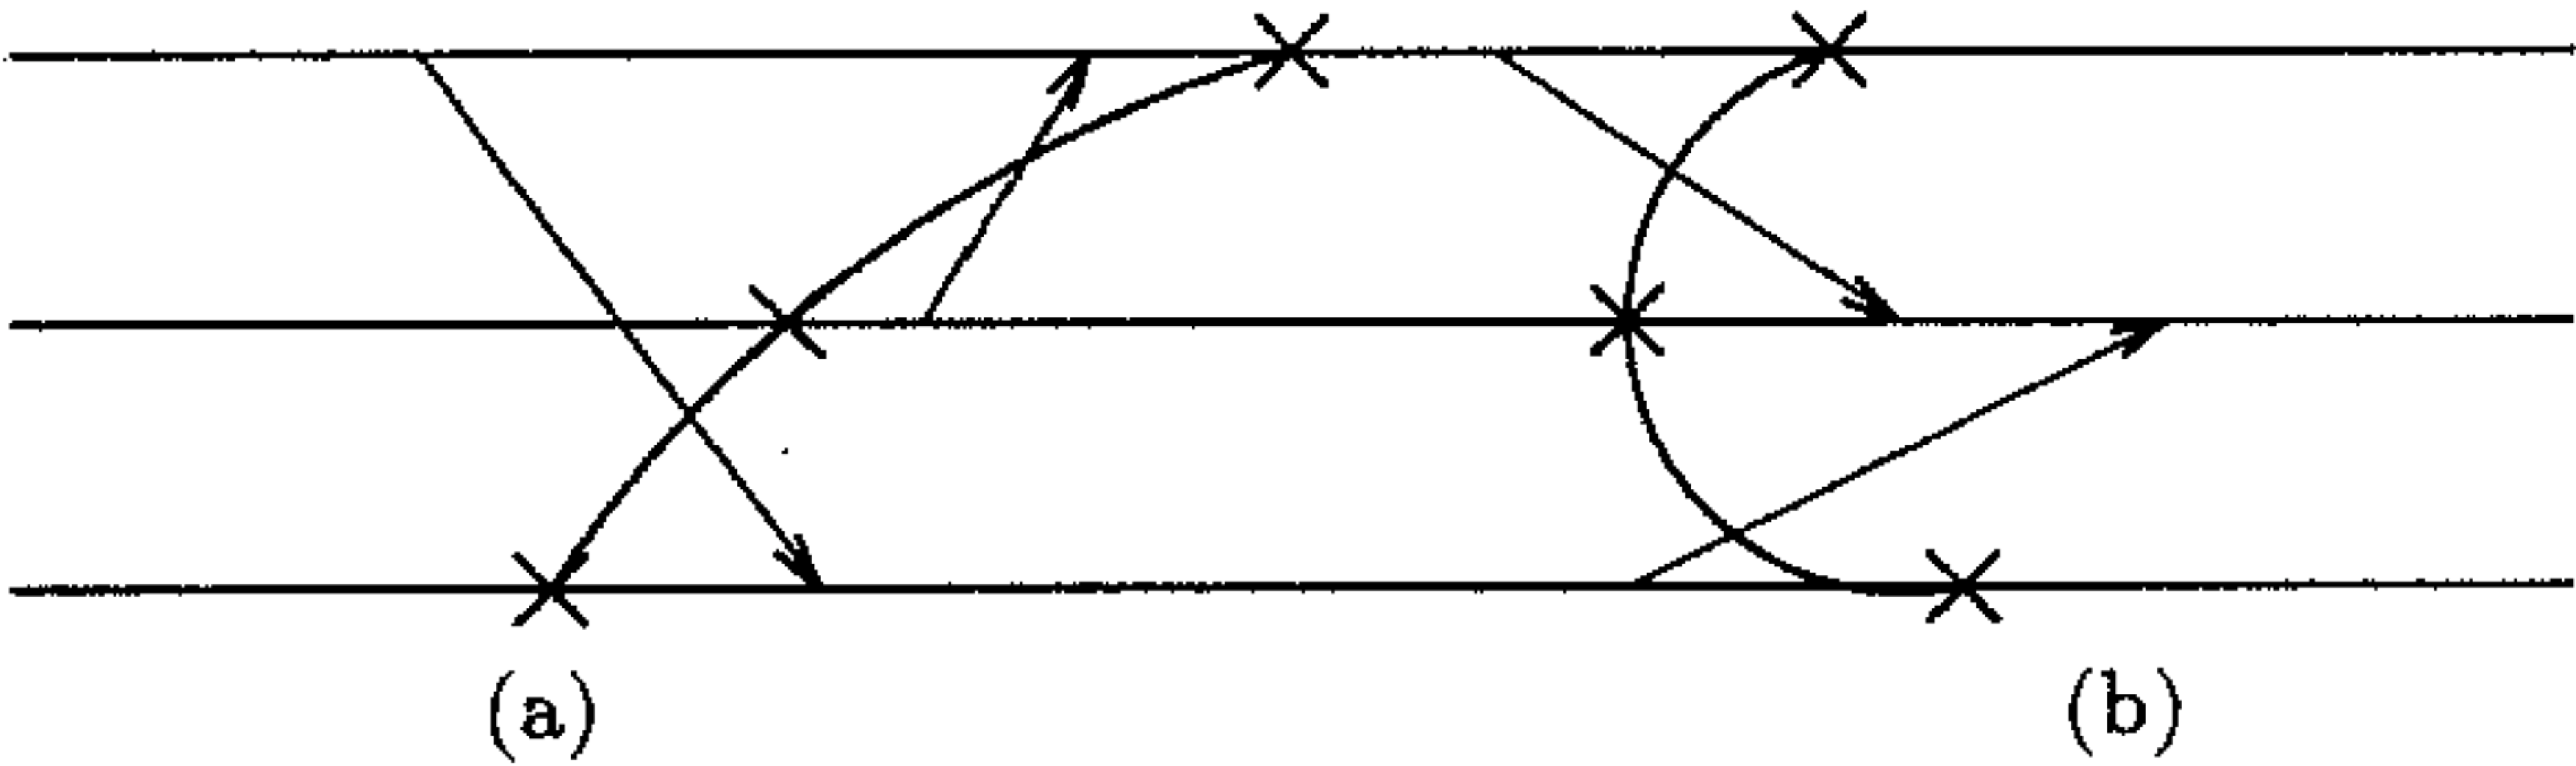
\includegraphics[width=0.8\textwidth]{def_async_sys.pdf}
%  \caption{ \cite{Panangaden1992} }
%\label{pic:fismahistorical}
%\end{figure}
Nachfolgend wird in diesem Kapitel beispielhaft erläutert, wie die Problematik des \textit{cheating husbands}-Rätsel für die Fälle der asynchronen und synchronen Übertragung behandelt werden.

%########################################################################################
% Section: Wissen in asynchronen Systemen
%########################################################################################
\subsection{Wissen in asynchronen Systemen}
\label{wissen_sync}
Für die asynchronen Systeme gibt es einen Zusatz in dem Rätsel der \textit{cheating husbands} (\cite{moses1986cheating} et al.). Es beginnt damit, dass Henrietta I verstirbt und damit ihre Tochter (Henrietta II) die Herrschaft von Mamajorca übernimmt. Der letzte Wunsch ihrer Mutter war es, dass Benachrichtungssystem für betrogene Ehefrauen fort zu führen. \\\\
Die Tochter kam der bitte ihrer Mutter nach. Jedoch vollführte sie eine Verbesserung des Systems. Um die Kommunikation zu erleichtern lies Henrietta II Briefkästen an jedem Haushalt in der ganzen Stadt anbringen. Nach dem errichten lies die Königin als erstes einen Brief an alle ausliefern in dem die Neuerungen erläutert wurden und die Eigenschaften des neuen Systems veranschaulicht wurden. Die erste Eigenschaft besagt, dass jeder Brief den die Königin verschickt, wird garantiert, zu einem \textit{nicht vorhersagbaren Zeitpunkt}, eine der Frauen erreichen. Somit ist die zweite Eigenschaft ableitbar aus der ersten. Sie besagt lediglich, dass keine Ankündigungen mehr auf dem Marktplatz gemacht werden müssten.\\\\
Der grundsätzliche Gedanke ist der gleiche. D.h. nach Erhalt der Nachricht wird der untreue Ehemann in der folgenden Nacht erschossen. Aufgrund des zeitversetzten Zustellens der Nachricht gibt es Zustände in einem System, welche nicht vorhersagbar sind. Jenes Problem wird nachfolgend in Theorem \ref{theo_async_1} erläutert.
\begin{theorem}[vgl. Theorem 2, \cite{moses1986cheating} S. 168]
\label{theo_async_1}
Wenn mehr wie ein untreuer Ehemann existiert und die originalen Anweisungen gelten,so sind  diese über einen asynchronen Kanal zu versenden, somit wird kein Ehemann erschossen.
\end{theorem}
\begin{proof}
Der Beweis ist durch Veranschaulichung des Ablaufes leicht zu erbringen. Durch die asynchrone Verteilung der Briefe und die Tatsache das es eine eventuelle Verteilung dieser Briefe gibt handelt es sich um "eventual common knowledge" (siehe Kap. \ref{GemeinsamesWissen}). Wird nun ein Brief von der Königin versendet, erhält jede Frau eventuell den Brief, der für sie bestimmt war und die besagt Frau weiß ebenfalls, dass es eventuell noch weitere Frauen gibt, die einen Brief erhalten haben könnten. Es gibt keine Sicherheit um für die Frauen um fest zu stellen, ob ihr Ehemann zweifelsfrei einer der untreuen ist. Zweifelsfrei kann sich dies deshalb nicht sagen lassen, da die Frau nicht weiß ob die ruhigen Nächte auf der Tatsache basieren, dass die anderen Briefe noch nicht zugestellt wurden oder ob es eine Reaktion andere Frauen auf den Erhalt eines Briefes ist.
\end{proof}
Aus dem Beweis resultiert, dass sich die Frauen auf Grund der Unsicherheit nie dazu entschließen würden, ihren Gemahlen zu erschießen, denn es könnte sich ja auch um einen Irrtum handeln, da noch nicht alle Briefe zugestellt wurden.
\begin{definition}
\begin{itemize}
\item (a,c) $\vDash \phi$ genau dann, wenn $\phi$ wahr ist in einem Schnitt c von der asynchronen Ausführung a.
\item (a,c) $\vDash K_i(\phi)$, genau dann, wenn 
$\forall(a',c'), ((a',c') \sim_i (a,c) \implies (a',c') \vDash \phi)$
\item (a,c) $\vDash E^0(\phi)$, genau dann, wenn (a,c) $\vDash \phi$
\item (a,c) $\vDash E^1(\phi)$, genau dann, wenn (a,c) $\vDash\land_{i\in N}K_i(\phi)$
\item (a,c) $\vDash E^{k+1}(\phi)$ mit $k\ge 1$, falls (a,c) $\vDash\land_{i\in N}K_i(E^k(\phi))$ mit $k\ge 1$
\item (a,c) $\vDash C(\phi)$, genau dann, wenn (a,c) $\vDash$ den größten Fixpunkt erfüllt mit $X=(E(X)\wedge \phi)$ gilt, $C(\phi) \land_{k\in Z^*}E^k(\phi)$
\end{itemize}
\end{definition}
Abbildung \ref{unsichereAbsprache} zeigt genau diesen Sachverhalt.

\begin{figure}
	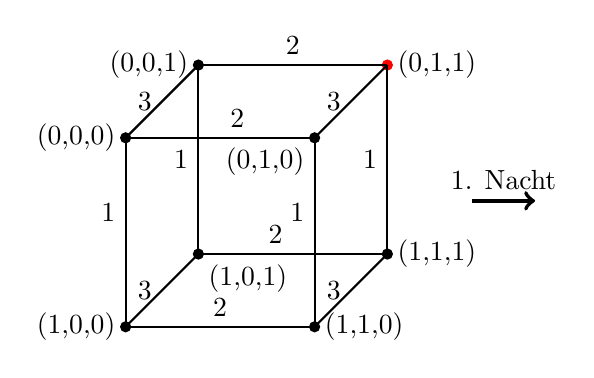
\begin{tikzpicture}[thick,scale=0.2]
	\coordinate[label={180:\text{(1,0,0)}}] (UVL) at (0,0,12);
	\coordinate[label={0:\text{(1,1,0)}}] (UVR) at (12,0,12);
	\coordinate[label={180:\text{(0,0,0)}}] (OVL) at (0,12,12);
	\coordinate[label={-120:\text{(0,1,0)}}] (OVR) at (12,12,12);
	\coordinate[label={-86:\text{(1,0,1)}}] (UHL) at (0,0,0);
	\coordinate[label={0:\text{(1,1,1)}}] (UHR) at (12,0,0);
	\coordinate[label={180:\text{(0,0,1)}}] (OHL) at (0,12,0);
	\coordinate[label={0:\text{(0,1,1)}}] (OHR) at (12,12,0);
	
	\draw[fill=black] (UVL) circle (8pt);
	\draw[fill=black] (UVR) circle (8pt);
	\draw[fill=black] (OVL) circle (8pt);
	\draw[fill=black] (OVR) circle (8pt);
	\draw[fill=black] (UHL) circle (8pt);
	\draw[fill=black] (UHR) circle (8pt);
	\draw[fill=black] (OHL) circle (8pt);
	\filldraw[color=red] (OHR) circle (8pt);
	
	\draw (UVL) -- node[above] {2} (UVR);
	\draw (UVL) -- node[above left] {1} (OVL);
	\draw (UVL) -- node[left] {3} (UHL);
	\draw (OVR) -- node[above right] {2} (OVL);
	\draw (OVR) -- node[left] {3} (OHR);
	\draw (OVR) -- node[above left] {1} (UVR);
	\draw (OHL) -- node[left] {3} (OVL);
	\draw (OHL) -- node[above] {2} (OHR);
	\draw (OHL) -- node[left] {1} (UHL);
	\draw (UHR) -- node[left] {3} (UVR);
	\draw (UHR) -- node[left] {1} (OHR);
	\draw (UHR) -- node[above left] {2} (UHL);	
	
	\draw[line width=1.5pt,->] (22,8,12) -- node[above] {1. Nacht} (26,8,12); 	
	\end{tikzpicture}
	\qquad
	\hspace*{-0.7cm}
	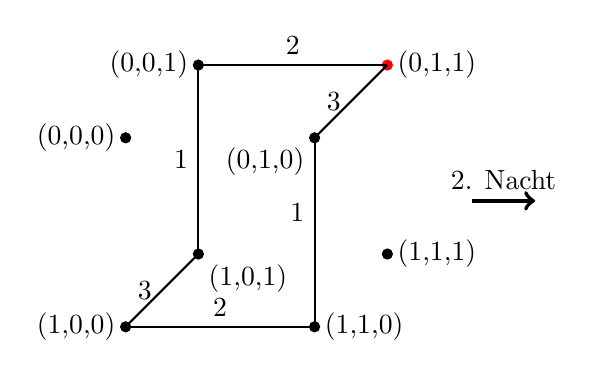
\begin{tikzpicture}[thick,scale=0.2]
	\coordinate[label={180:\text{(1,0,0)}}] (UVL) at (0,0,12);
	\coordinate[label={0:\text{(1,1,0)}}] (UVR) at (12,0,12);
	\coordinate[label={180:\text{(0,0,0)}}] (OVL) at (0,12,12);
	\coordinate[label={-120:\text{(0,1,0)}}] (OVR) at (12,12,12);
	\coordinate[label={-86:\text{(1,0,1)}}] (UHL) at (0,0,0);
	\coordinate[label={0:\text{(1,1,1)}}] (UHR) at (12,0,0);
	\coordinate[label={180:\text{(0,0,1)}}] (OHL) at (0,12,0);
	\coordinate[label={0:\text{(0,1,1)}}] (OHR) at (12,12,0);
	
	\draw[fill=black] (UVL) circle (8pt);
	\draw[fill=black] (UVR) circle (8pt);
	\draw[fill=black] (OVL) circle (8pt);
	\draw[fill=black] (OVR) circle (8pt);
	\draw[fill=black] (UHL) circle (8pt);
	\draw[fill=black] (UHR) circle (8pt);
	\draw[fill=black] (OHL) circle (8pt);
	\filldraw[color=red] (OHR) circle (8pt);	
	
	\draw (UVL) -- node[above] {2} (UVR);
	\draw (UVL) -- node[left] {3} (UHL);
	\draw (OVR) -- node[left] {3} (OHR);
	\draw (OVR) -- node[above left] {1} (UVR);
	\draw (OHL) -- node[above] {2} (OHR);
	\draw (OHL) -- node[left] {1} (UHL);
	\draw[line width=1.5pt,->] (22,8,12) -- node[above] {2. Nacht} (26,8,12); 		
	\end{tikzpicture}
	\centering	
	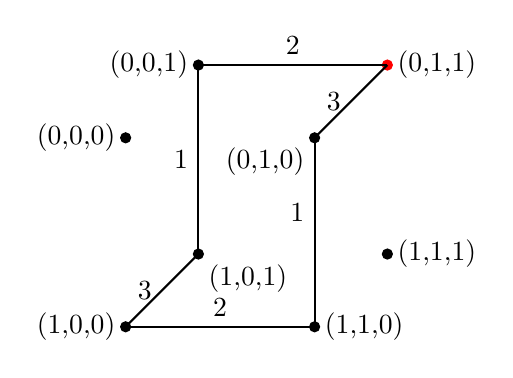
\begin{tikzpicture}[thick,scale=0.2]
	\coordinate[label={180:\text{(1,0,0)}}] (UVL) at (0,0,12);
	\coordinate[label={0:\text{(1,1,0)}}] (UVR) at (12,0,12);
	\coordinate[label={180:\text{(0,0,0)}}] (OVL) at (0,12,12);
	\coordinate[label={-120:\text{(0,1,0)}}] (OVR) at (12,12,12);
	\coordinate[label={-86:\text{(1,0,1)}}] (UHL) at (0,0,0);
	\coordinate[label={0:\text{(1,1,1)}}] (UHR) at (12,0,0);
	\coordinate[label={180:\text{(0,0,1)}}] (OHL) at (0,12,0);
	\coordinate[label={0:\text{(0,1,1)}}] (OHR) at (12,12,0);
	
	\draw[fill=black] (UVL) circle (8pt);
	\draw[fill=black] (UVR) circle (8pt);
	\draw[fill=black] (OVL) circle (8pt);
	\draw[fill=black] (OVR) circle (8pt);
	\draw[fill=black] (UHL) circle (8pt);
	\draw[fill=black] (UHR) circle (8pt);
	\draw[fill=black] (OHL) circle (8pt);
	\filldraw[color=red] (OHR) circle (8pt);	
	
	\draw (UVL) -- node[above] {2} (UVR);
	\draw (UVL) -- node[left] {3} (UHL);
	\draw (OVR) -- node[left] {3} (OHR);
	\draw (OVR) -- node[above left] {1} (UVR);
	\draw (OHL) -- node[above] {2} (OHR);
	\draw (OHL) -- node[left] {1} (UHL);	
	\end{tikzpicture}
	\caption{Übergang vom ersten zum zweiten Tag im \textit{cheating husbands}-Rätsels mit ungenügender Kommunikation ausgehend vom Zustand (0,1,1).}
	\label{unsichereAbsprache}
\end{figure}
%########################################################################################
% Section: Wissen in synchronen Systemen
%########################################################################################

\subsection{Wissen in synchronen Systemen}
\label{wissen_async}




\begin{satz}[vgl. \cite{moses1986cheating} S. 168]
\label{pythagorean}
Wenn mehr wie ein untreuer Ehemann existiert und die originalen Anweisungen sind, diese über einen asynchronen Kanal zu versenden, dann wird kein Ehemann erschossen.
\end{satz}

\begin{figure}
\centering
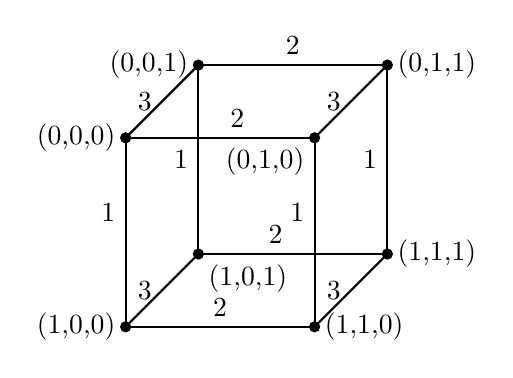
\begin{tikzpicture}[thick,scale=0.2]
\coordinate[label={180:\text{(1,0,0)}}] (UVL) at (0,0,12);
\coordinate[label={0:\text{(1,1,0)}}] (UVR) at (12,0,12);
\coordinate[label={180:\text{(0,0,0)}}] (OVL) at (0,12,12);
\coordinate[label={-120:\text{(0,1,0)}}] (OVR) at (12,12,12);
\coordinate[label={-86:\text{(1,0,1)}}] (UHL) at (0,0,0);
\coordinate[label={0:\text{(1,1,1)}}] (UHR) at (12,0,0);
\coordinate[label={180:\text{(0,0,1)}}] (OHL) at (0,12,0);
\coordinate[label={0:\text{(0,1,1)}}] (OHR) at (12,12,0);

\draw[fill=black] (UVL) circle (8pt);
\draw[fill=black] (UVR) circle (8pt);
\draw[fill=black] (OVL) circle (8pt);
\draw[fill=black] (OVR) circle (8pt);
\draw[fill=black] (UHL) circle (8pt);
\draw[fill=black] (UHR) circle (8pt);
\draw[fill=black] (OHL) circle (8pt);
\filldraw[color=black] (OHR) circle (8pt);

\draw (UVL) -- node[above] {2} (UVR);
\draw (UVL) -- node[above left] {1} (OVL);
\draw (UVL) -- node[left] {3} (UHL);
\draw (OVR) -- node[above right] {2} (OVL);
\draw (OVR) -- node[left] {3} (OHR);
\draw (OVR) -- node[above left] {1} (UVR);
\draw (OHL) -- node[left] {3} (OVL);
\draw (OHL) -- node[above] {2} (OHR);
\draw (OHL) -- node[left] {1} (UHL);
\draw (UHR) -- node[left] {3} (UVR);
\draw (UHR) -- node[left] {1} (OHR);
\draw (UHR) -- node[above left] {2} (UHL);
\end{tikzpicture}
\caption{Ausgangssituation des \textit{cheating husbands}-Rätsels}
\label{ausgang}
\end{figure}
